\usepackage{graphicx}

While the greedy algorithm allows us to find near optimals for problems where we have perfect information about the
problem case like the job utility, this may be private information that the job owner doesnt want to reveal also
server would want to get paid for that work that they do. \\
We propose a iterative auctions that occurs before any processing is done and allows the job owner doesnt have to reveal
it's true utility. In normal VCG auctions, then the auctioneer will solve the problem to maximise the social welfare
(total utility of allocated jobs) and
must find the optimal solution. Then for each job and server, the job or server is removed from the problem case and the
optimal is solved for that as well with the server's revenue it is paid and the job's cost being the social welfare of
the optimal solution minus the social welfare of the optimal without the job or server. This is extremely slow and
unscalable because of this so is not used often however has the properties that it is individually rational, truthful
bidding and incentive compatible. \\

\subsection{Proposed Iterative Auction}\label{subsec:proposed-iterative-auction}
Our iterative auctions uses the idea of VCG so that when a job asks to run on a server then the server will calculate
current revenue of the jobs running minus the revenue if the new job must be running on the server plus a price increase
factor. This is then the price for the job to run on the server as the new allocation with the job would be to a greater
revenue for the server than is currently allocated.

\subsection{Iterative Auction Properties}\label{subsec:iterative-auction-properties}
Auctions mainly consider four different properties that are important: Economic Efficiency, Individual Rational,
Incentive Compatibility and Budget Balance. We believe that our iterative auction is Budget Balanced and Individual rational
and possibly economic efficient however not incentive compatible. \\

\subsubsection{Proving budget balance for auction}
Budget balance is that the sum of revenue and the sum of prices is zero, as our algorithm doesnt require an auctioneer
then budget balance is true. The algorithm can be run with a centralised auctioneer or in a decentralised manner such that
jobs don't need to be aware of each others existence with a job only directly communicating with the server.
\subsubsection{Proving individual rational}
The utility of all partitions are non-negative therefore the sum of all server revenue $\geq$ the sum of revenue without
jobs. So the revenue of a job must be non-negative. %% TODO
\subsubsection{Economic efficient and Incentive compatible}
Our algorithm is not economically efficient or incentive compatible due a server only considering itself in choosing its
price and is unaware of the price being charged by other servers. Because of this then the allocation of jobs to server
may not be optimal resulting in a suboptimal economic efficient however in over 50%

\subsection{Iterative Auction algorithm}\label{subsec:iterative-auction-algorithm}
\begin{lstlisting}[language=Python]
unallocated_jobs = jobs
while len(unallocated_jobs):
    # Select a job, can be at random
    job = unallocated_jobs[0]

    # Calculate the minimum job price on all of the servers
    job_price, allocation_info = min((evaluate_job_price(job, server, epsilon=epsilon)
                                     for server in servers), key=lambda bid: bid[0])
        # Check if the job can pay the minimum price
        if job_price <= job.utility:
            # Uses the allocation info to create the new allocation on the selected server
            allocate_job(job_price, job, allocation_info, unallocated_jobs)
        else:
            # Remove job as the job can be run ever at a price lower than the job's value utility
            unallocated_jobs.remove(job)
\end{lstlisting}

\section{Iterative Auction Results}\label{sec:auctions-results}
\begin{figure}[H]
    \centering
    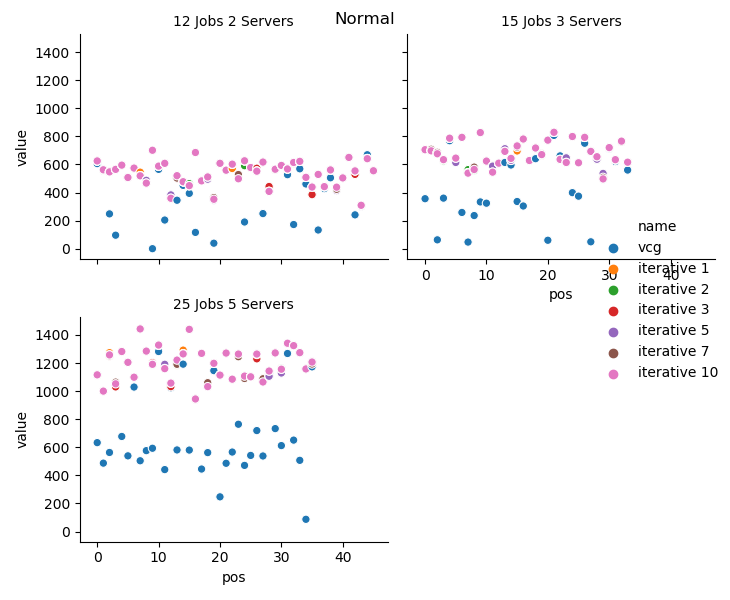
\includegraphics[width=1\linewidth]{./images/single_price_auction_results.png}
    \caption{Multiple Price auction results}
\end{figure}
\begin{figure}[H]
    \centering
    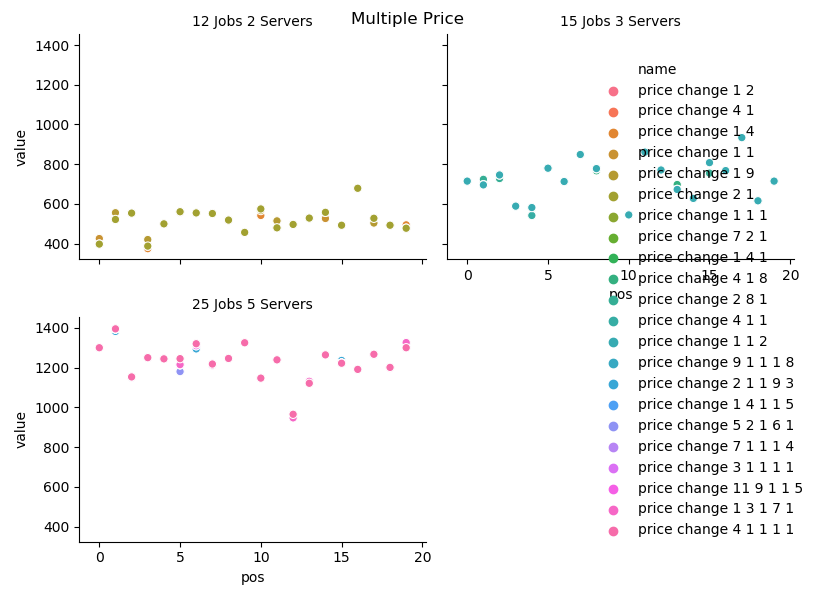
\includegraphics[width=1\linewidth]{./images/multiple_price_auction_results.png}
    \caption{Multiple Price auction results}
\end{figure}
\begin{figure}[H]
    \centering
    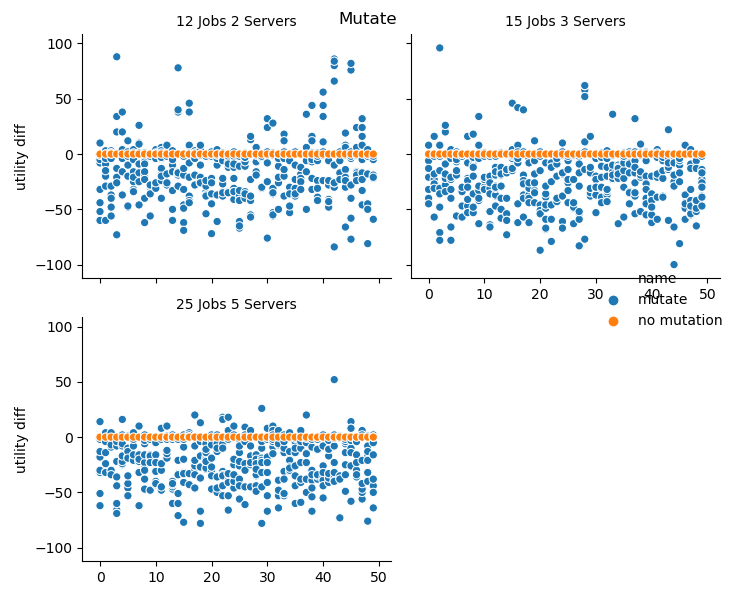
\includegraphics[width=1\linewidth]{./images/mutated_auction.png}
    \caption{Mutated Jobs and servers in auctions}
\end{figure}